
% Default to the notebook output style




% Inherit from the specified cell style.





\documentclass{article}



    \usepackage{graphicx} % Used to insert images
    \usepackage{adjustbox} % Used to constrain images to a maximum size
    \usepackage{color} % Allow colors to be defined
    \usepackage{enumerate} % Needed for markdown enumerations to work
    \usepackage{geometry} % Used to adjust the document margins
    \usepackage{amsmath} % Equations
    \usepackage{amssymb} % Equations
    \usepackage{eurosym} % defines \euro
    \usepackage[mathletters]{ucs} % Extended unicode (utf-8) support
    \usepackage[utf8x]{inputenc} % Allow utf-8 characters in the tex document
    \usepackage{fancyvrb} % verbatim replacement that allows latex
    \usepackage{grffile} % extends the file name processing of package graphics
                         % to support a larger range
    % The hyperref package gives us a pdf with properly built
    % internal navigation ('pdf bookmarks' for the table of contents,
    % internal cross-reference links, web links for URLs, etc.)
    \usepackage{hyperref}
    \usepackage{longtable} % longtable support required by pandoc >1.10
    \usepackage{booktabs}  % table support for pandoc > 1.12.2




    \definecolor{orange}{cmyk}{0,0.4,0.8,0.2}
    \definecolor{darkorange}{rgb}{.71,0.21,0.01}
    \definecolor{darkgreen}{rgb}{.12,.54,.11}
    \definecolor{myteal}{rgb}{.26, .44, .56}
    \definecolor{gray}{gray}{0.45}
    \definecolor{lightgray}{gray}{.95}
    \definecolor{mediumgray}{gray}{.8}
    \definecolor{inputbackground}{rgb}{.95, .95, .85}
    \definecolor{outputbackground}{rgb}{.95, .95, .95}
    \definecolor{traceback}{rgb}{1, .95, .95}
    % ansi colors
    \definecolor{red}{rgb}{.6,0,0}
    \definecolor{green}{rgb}{0,.65,0}
    \definecolor{brown}{rgb}{0.6,0.6,0}
    \definecolor{blue}{rgb}{0,.145,.698}
    \definecolor{purple}{rgb}{.698,.145,.698}
    \definecolor{cyan}{rgb}{0,.698,.698}
    \definecolor{lightgray}{gray}{0.5}

    % bright ansi colors
    \definecolor{darkgray}{gray}{0.25}
    \definecolor{lightred}{rgb}{1.0,0.39,0.28}
    \definecolor{lightgreen}{rgb}{0.48,0.99,0.0}
    \definecolor{lightblue}{rgb}{0.53,0.81,0.92}
    \definecolor{lightpurple}{rgb}{0.87,0.63,0.87}
    \definecolor{lightcyan}{rgb}{0.5,1.0,0.83}

    % commands and environments needed by pandoc snippets
    % extracted from the output of `pandoc -s`
    \providecommand{\tightlist}{%
      \setlength{\itemsep}{0pt}\setlength{\parskip}{0pt}}
    \DefineVerbatimEnvironment{Highlighting}{Verbatim}{commandchars=\\\{\}}
    % Add ',fontsize=\small' for more characters per line
    \newenvironment{Shaded}{}{}
    \newcommand{\KeywordTok}[1]{\textcolor[rgb]{0.00,0.44,0.13}{\textbf{{#1}}}}
    \newcommand{\DataTypeTok}[1]{\textcolor[rgb]{0.56,0.13,0.00}{{#1}}}
    \newcommand{\DecValTok}[1]{\textcolor[rgb]{0.25,0.63,0.44}{{#1}}}
    \newcommand{\BaseNTok}[1]{\textcolor[rgb]{0.25,0.63,0.44}{{#1}}}
    \newcommand{\FloatTok}[1]{\textcolor[rgb]{0.25,0.63,0.44}{{#1}}}
    \newcommand{\CharTok}[1]{\textcolor[rgb]{0.25,0.44,0.63}{{#1}}}
    \newcommand{\StringTok}[1]{\textcolor[rgb]{0.25,0.44,0.63}{{#1}}}
    \newcommand{\CommentTok}[1]{\textcolor[rgb]{0.38,0.63,0.69}{\textit{{#1}}}}
    \newcommand{\OtherTok}[1]{\textcolor[rgb]{0.00,0.44,0.13}{{#1}}}
    \newcommand{\AlertTok}[1]{\textcolor[rgb]{1.00,0.00,0.00}{\textbf{{#1}}}}
    \newcommand{\FunctionTok}[1]{\textcolor[rgb]{0.02,0.16,0.49}{{#1}}}
    \newcommand{\RegionMarkerTok}[1]{{#1}}
    \newcommand{\ErrorTok}[1]{\textcolor[rgb]{1.00,0.00,0.00}{\textbf{{#1}}}}
    \newcommand{\NormalTok}[1]{{#1}}

    % Define a nice break command that doesn't care if a line doesn't already
    % exist.
    \def\br{\hspace*{\fill} \\* }
    % Math Jax compatability definitions
    \def\gt{>}
    \def\lt{<}
    % Document parameters
    \title{Analyzing the NYC Subway Dataset}




    % Pygments definitions

\makeatletter
\def\PY@reset{\let\PY@it=\relax \let\PY@bf=\relax%
    \let\PY@ul=\relax \let\PY@tc=\relax%
    \let\PY@bc=\relax \let\PY@ff=\relax}
\def\PY@tok#1{\csname PY@tok@#1\endcsname}
\def\PY@toks#1+{\ifx\relax#1\empty\else%
    \PY@tok{#1}\expandafter\PY@toks\fi}
\def\PY@do#1{\PY@bc{\PY@tc{\PY@ul{%
    \PY@it{\PY@bf{\PY@ff{#1}}}}}}}
\def\PY#1#2{\PY@reset\PY@toks#1+\relax+\PY@do{#2}}

\expandafter\def\csname PY@tok@gd\endcsname{\def\PY@tc##1{\textcolor[rgb]{0.63,0.00,0.00}{##1}}}
\expandafter\def\csname PY@tok@gu\endcsname{\let\PY@bf=\textbf\def\PY@tc##1{\textcolor[rgb]{0.50,0.00,0.50}{##1}}}
\expandafter\def\csname PY@tok@gt\endcsname{\def\PY@tc##1{\textcolor[rgb]{0.00,0.27,0.87}{##1}}}
\expandafter\def\csname PY@tok@gs\endcsname{\let\PY@bf=\textbf}
\expandafter\def\csname PY@tok@gr\endcsname{\def\PY@tc##1{\textcolor[rgb]{1.00,0.00,0.00}{##1}}}
\expandafter\def\csname PY@tok@cm\endcsname{\let\PY@it=\textit\def\PY@tc##1{\textcolor[rgb]{0.25,0.50,0.50}{##1}}}
\expandafter\def\csname PY@tok@vg\endcsname{\def\PY@tc##1{\textcolor[rgb]{0.10,0.09,0.49}{##1}}}
\expandafter\def\csname PY@tok@m\endcsname{\def\PY@tc##1{\textcolor[rgb]{0.40,0.40,0.40}{##1}}}
\expandafter\def\csname PY@tok@mh\endcsname{\def\PY@tc##1{\textcolor[rgb]{0.40,0.40,0.40}{##1}}}
\expandafter\def\csname PY@tok@go\endcsname{\def\PY@tc##1{\textcolor[rgb]{0.53,0.53,0.53}{##1}}}
\expandafter\def\csname PY@tok@ge\endcsname{\let\PY@it=\textit}
\expandafter\def\csname PY@tok@vc\endcsname{\def\PY@tc##1{\textcolor[rgb]{0.10,0.09,0.49}{##1}}}
\expandafter\def\csname PY@tok@il\endcsname{\def\PY@tc##1{\textcolor[rgb]{0.40,0.40,0.40}{##1}}}
\expandafter\def\csname PY@tok@cs\endcsname{\let\PY@it=\textit\def\PY@tc##1{\textcolor[rgb]{0.25,0.50,0.50}{##1}}}
\expandafter\def\csname PY@tok@cp\endcsname{\def\PY@tc##1{\textcolor[rgb]{0.74,0.48,0.00}{##1}}}
\expandafter\def\csname PY@tok@gi\endcsname{\def\PY@tc##1{\textcolor[rgb]{0.00,0.63,0.00}{##1}}}
\expandafter\def\csname PY@tok@gh\endcsname{\let\PY@bf=\textbf\def\PY@tc##1{\textcolor[rgb]{0.00,0.00,0.50}{##1}}}
\expandafter\def\csname PY@tok@ni\endcsname{\let\PY@bf=\textbf\def\PY@tc##1{\textcolor[rgb]{0.60,0.60,0.60}{##1}}}
\expandafter\def\csname PY@tok@nl\endcsname{\def\PY@tc##1{\textcolor[rgb]{0.63,0.63,0.00}{##1}}}
\expandafter\def\csname PY@tok@nn\endcsname{\let\PY@bf=\textbf\def\PY@tc##1{\textcolor[rgb]{0.00,0.00,1.00}{##1}}}
\expandafter\def\csname PY@tok@no\endcsname{\def\PY@tc##1{\textcolor[rgb]{0.53,0.00,0.00}{##1}}}
\expandafter\def\csname PY@tok@na\endcsname{\def\PY@tc##1{\textcolor[rgb]{0.49,0.56,0.16}{##1}}}
\expandafter\def\csname PY@tok@nb\endcsname{\def\PY@tc##1{\textcolor[rgb]{0.00,0.50,0.00}{##1}}}
\expandafter\def\csname PY@tok@nc\endcsname{\let\PY@bf=\textbf\def\PY@tc##1{\textcolor[rgb]{0.00,0.00,1.00}{##1}}}
\expandafter\def\csname PY@tok@nd\endcsname{\def\PY@tc##1{\textcolor[rgb]{0.67,0.13,1.00}{##1}}}
\expandafter\def\csname PY@tok@ne\endcsname{\let\PY@bf=\textbf\def\PY@tc##1{\textcolor[rgb]{0.82,0.25,0.23}{##1}}}
\expandafter\def\csname PY@tok@nf\endcsname{\def\PY@tc##1{\textcolor[rgb]{0.00,0.00,1.00}{##1}}}
\expandafter\def\csname PY@tok@si\endcsname{\let\PY@bf=\textbf\def\PY@tc##1{\textcolor[rgb]{0.73,0.40,0.53}{##1}}}
\expandafter\def\csname PY@tok@s2\endcsname{\def\PY@tc##1{\textcolor[rgb]{0.73,0.13,0.13}{##1}}}
\expandafter\def\csname PY@tok@vi\endcsname{\def\PY@tc##1{\textcolor[rgb]{0.10,0.09,0.49}{##1}}}
\expandafter\def\csname PY@tok@nt\endcsname{\let\PY@bf=\textbf\def\PY@tc##1{\textcolor[rgb]{0.00,0.50,0.00}{##1}}}
\expandafter\def\csname PY@tok@nv\endcsname{\def\PY@tc##1{\textcolor[rgb]{0.10,0.09,0.49}{##1}}}
\expandafter\def\csname PY@tok@s1\endcsname{\def\PY@tc##1{\textcolor[rgb]{0.73,0.13,0.13}{##1}}}
\expandafter\def\csname PY@tok@kd\endcsname{\let\PY@bf=\textbf\def\PY@tc##1{\textcolor[rgb]{0.00,0.50,0.00}{##1}}}
\expandafter\def\csname PY@tok@sh\endcsname{\def\PY@tc##1{\textcolor[rgb]{0.73,0.13,0.13}{##1}}}
\expandafter\def\csname PY@tok@sc\endcsname{\def\PY@tc##1{\textcolor[rgb]{0.73,0.13,0.13}{##1}}}
\expandafter\def\csname PY@tok@sx\endcsname{\def\PY@tc##1{\textcolor[rgb]{0.00,0.50,0.00}{##1}}}
\expandafter\def\csname PY@tok@bp\endcsname{\def\PY@tc##1{\textcolor[rgb]{0.00,0.50,0.00}{##1}}}
\expandafter\def\csname PY@tok@c1\endcsname{\let\PY@it=\textit\def\PY@tc##1{\textcolor[rgb]{0.25,0.50,0.50}{##1}}}
\expandafter\def\csname PY@tok@kc\endcsname{\let\PY@bf=\textbf\def\PY@tc##1{\textcolor[rgb]{0.00,0.50,0.00}{##1}}}
\expandafter\def\csname PY@tok@c\endcsname{\let\PY@it=\textit\def\PY@tc##1{\textcolor[rgb]{0.25,0.50,0.50}{##1}}}
\expandafter\def\csname PY@tok@mf\endcsname{\def\PY@tc##1{\textcolor[rgb]{0.40,0.40,0.40}{##1}}}
\expandafter\def\csname PY@tok@err\endcsname{\def\PY@bc##1{\setlength{\fboxsep}{0pt}\fcolorbox[rgb]{1.00,0.00,0.00}{1,1,1}{\strut ##1}}}
\expandafter\def\csname PY@tok@mb\endcsname{\def\PY@tc##1{\textcolor[rgb]{0.40,0.40,0.40}{##1}}}
\expandafter\def\csname PY@tok@ss\endcsname{\def\PY@tc##1{\textcolor[rgb]{0.10,0.09,0.49}{##1}}}
\expandafter\def\csname PY@tok@sr\endcsname{\def\PY@tc##1{\textcolor[rgb]{0.73,0.40,0.53}{##1}}}
\expandafter\def\csname PY@tok@mo\endcsname{\def\PY@tc##1{\textcolor[rgb]{0.40,0.40,0.40}{##1}}}
\expandafter\def\csname PY@tok@kn\endcsname{\let\PY@bf=\textbf\def\PY@tc##1{\textcolor[rgb]{0.00,0.50,0.00}{##1}}}
\expandafter\def\csname PY@tok@mi\endcsname{\def\PY@tc##1{\textcolor[rgb]{0.40,0.40,0.40}{##1}}}
\expandafter\def\csname PY@tok@gp\endcsname{\let\PY@bf=\textbf\def\PY@tc##1{\textcolor[rgb]{0.00,0.00,0.50}{##1}}}
\expandafter\def\csname PY@tok@o\endcsname{\def\PY@tc##1{\textcolor[rgb]{0.40,0.40,0.40}{##1}}}
\expandafter\def\csname PY@tok@kr\endcsname{\let\PY@bf=\textbf\def\PY@tc##1{\textcolor[rgb]{0.00,0.50,0.00}{##1}}}
\expandafter\def\csname PY@tok@s\endcsname{\def\PY@tc##1{\textcolor[rgb]{0.73,0.13,0.13}{##1}}}
\expandafter\def\csname PY@tok@kp\endcsname{\def\PY@tc##1{\textcolor[rgb]{0.00,0.50,0.00}{##1}}}
\expandafter\def\csname PY@tok@w\endcsname{\def\PY@tc##1{\textcolor[rgb]{0.73,0.73,0.73}{##1}}}
\expandafter\def\csname PY@tok@kt\endcsname{\def\PY@tc##1{\textcolor[rgb]{0.69,0.00,0.25}{##1}}}
\expandafter\def\csname PY@tok@ow\endcsname{\let\PY@bf=\textbf\def\PY@tc##1{\textcolor[rgb]{0.67,0.13,1.00}{##1}}}
\expandafter\def\csname PY@tok@sb\endcsname{\def\PY@tc##1{\textcolor[rgb]{0.73,0.13,0.13}{##1}}}
\expandafter\def\csname PY@tok@k\endcsname{\let\PY@bf=\textbf\def\PY@tc##1{\textcolor[rgb]{0.00,0.50,0.00}{##1}}}
\expandafter\def\csname PY@tok@se\endcsname{\let\PY@bf=\textbf\def\PY@tc##1{\textcolor[rgb]{0.73,0.40,0.13}{##1}}}
\expandafter\def\csname PY@tok@sd\endcsname{\let\PY@it=\textit\def\PY@tc##1{\textcolor[rgb]{0.73,0.13,0.13}{##1}}}

\def\PYZbs{\char`\\}
\def\PYZus{\char`\_}
\def\PYZob{\char`\{}
\def\PYZcb{\char`\}}
\def\PYZca{\char`\^}
\def\PYZam{\char`\&}
\def\PYZlt{\char`\<}
\def\PYZgt{\char`\>}
\def\PYZsh{\char`\#}
\def\PYZpc{\char`\%}
\def\PYZdl{\char`\$}
\def\PYZhy{\char`\-}
\def\PYZsq{\char`\'}
\def\PYZdq{\char`\"}
\def\PYZti{\char`\~}
% for compatibility with earlier versions
\def\PYZat{@}
\def\PYZlb{[}
\def\PYZrb{]}
\makeatother


    % Exact colors from NB
    \definecolor{incolor}{rgb}{0.0, 0.0, 0.5}
    \definecolor{outcolor}{rgb}{0.545, 0.0, 0.0}




    % Prevent overflowing lines due to hard-to-break entities
    \sloppy
    % Setup hyperref package
    \hypersetup{
      breaklinks=true,  % so long urls are correctly broken across lines
      colorlinks=true,
      urlcolor=blue,
      linkcolor=darkorange,
      citecolor=darkgreen,
      }
    % Slightly bigger margins than the latex defaults

    \geometry{verbose,tmargin=1in,bmargin=1in,lmargin=1in,rmargin=1in}



    \begin{document}


    \maketitle




    Analyzing the NYC Subway Dataset

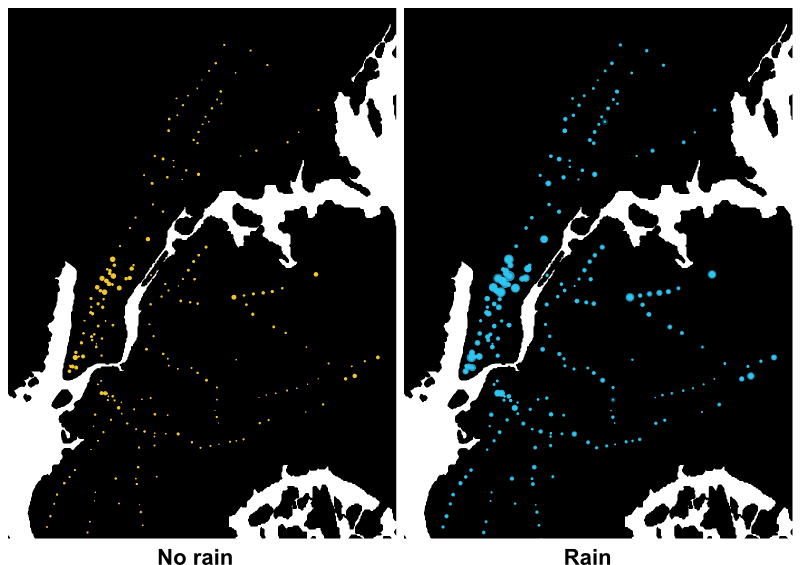
\includegraphics{rain_no_rain_v2.png}

FIG 1: The data plotted is the ENTRIESn\_hourly when it wasn't raining
(Left) and when it was raining (Right). Furthermore the data for when it
wasn't raining was scaled by the number of days it didn't rain, while
the data for when it was raining was scaled by the number of days it did
rain. The sizes of the dots represent the number of ENTRIESn\_hourly.

\subsubsection{Project Topics: Data Wrangling, Statistics, Machine
Learning, and Effective
Visualizations}\label{project-topics-data-wrangling-statistics-machine-learning-and-effective-visualizations}

This is the second project of the Udacity Data Analyst Nanodegree. In it
we analyze the NYC Subway Dataset to find out if more people take the
subway when it's raining than when it is not. It consists of two parts.
Part 1 of the project is to answer Problem sets 2, 3, and 4 of the
course Intro to Data Science on Udacity. This course gives an
introduction to many tools necessary for aspiring data scientists to
know, like exploratory analysis, data wrangling, interacting with large
datasets through sql, applying statistical tests, using machine learning
for predicting outcomes, and visualizing data. Part 2 is a reflection of
how the problem sets were solved and why specific statistical tests
might have been chosen. Combining these two parts I will try to guide
you through my thought process as I was solving the problem sets.

\begin{center}\rule{0.5\linewidth}{\linethickness}\end{center}

\subsubsection{The NYC Subway Dataset}\label{the-nyc-subway-dataset}

The NYC Subway dataset is a huge dataset consisting of over 100000 rows
and about 22 columns of data. The dataset has the number of entries and
exits registered by specific subway units at specific dates and at
specific times a day. Furthermore, it has weather related information at
these specific timestamps, like whether or not it was raining, whether
or not it was foggy, and many more. Below is a list of all the columns,
and for more information on what these specific parameters are see
\href{https://s3.amazonaws.com/uploads.hipchat.com/23756/665149/05bgLZqSsMycnkg/turnstile-weather-variables.pdf}{this
document}.

    \begin{Verbatim}[commandchars=\\\{\}]
{\color{incolor}In [{\color{incolor}17}]:} \PY{k+kn}{import} \PY{n+nn}{pandas} \PY{k+kn}{as} \PY{n+nn}{pd}
         \PY{n}{turnstile\PYZus{}weatherdata} \PY{o}{=} \PY{n}{pd}\PY{o}{.}\PY{n}{read\PYZus{}csv}\PY{p}{(}\PY{l+s}{\PYZdq{}}\PY{l+s}{./data/turnstile\PYZus{}data\PYZus{}master\PYZus{}with\PYZus{}weather.csv}\PY{l+s}{\PYZdq{}}\PY{p}{,}
                                             \PY{n}{sep}\PY{o}{=}\PY{l+s}{\PYZdq{}}\PY{l+s}{,}\PY{l+s}{\PYZdq{}}\PY{p}{)}

         \PY{c}{\PYZsh{} turnstile\PYZus{}weatherdata.take(1)}
         \PY{k}{for} \PY{n}{c} \PY{o+ow}{in} \PY{n}{turnstile\PYZus{}weatherdata}\PY{o}{.}\PY{n}{columns}\PY{o}{.}\PY{n}{values}\PY{p}{[}\PY{l+m+mi}{1}\PY{p}{:}\PY{p}{]}\PY{p}{:}
             \PY{k}{print} \PY{l+s}{\PYZdq{}}\PY{l+s+si}{\PYZpc{}s}\PY{l+s}{,}\PY{l+s}{\PYZdq{}} \PY{o}{\PYZpc{}} \PY{n}{c}\PY{p}{,}
\end{Verbatim}

    \begin{Verbatim}[commandchars=\\\{\}]
UNIT, DATEn, TIMEn, Hour, DESCn, ENTRIESn\_hourly, EXITSn\_hourly, maxpressurei, maxdewpti, mindewpti, minpressurei, meandewpti, meanpressurei, fog, rain, meanwindspdi, mintempi, meantempi, maxtempi, precipi, thunder,
    \end{Verbatim}

    Throughout this project and the Introduction to Data Science course, I
used a number of resources, besides the course material, to help me
answer some of the questions. Here you'll find a list of these
references, which might benefit you if you're ever in a situation where
you need to analyze a large dataset and want to do some statistical
tests on it. Furthermore, reading some of these links might actually
give you ideas for other things you could try on your dataset. \#\#\#\#
Visualizations and Inspiration *
\href{http://www.danielforsyth.me/mapping-nyc-taxi-data/}{Mapping NYC
Taxi Data} *
\href{http://basemaptutorial.readthedocs.org/en/latest/}{Basemap} *
\href{http://flowingdata.com/2009/11/12/how-to-make-a-us-county-thematic-map-using-free-tools/}{FlowingData}
* \href{http://maxberggren.se/2015/08/04/basemap/}{Working with Maps in
Python} *
\href{http://sensitivecities.com/so-youd-like-to-make-a-map-using-python-EN.html}{More
Working with Maps in Python}

\paragraph{Understanding the Statistical
Tests}\label{understanding-the-statistical-tests}

\begin{itemize}
\tightlist
\item
  \href{https://en.wikipedia.org/wiki/Mann\%E2\%80\%93Whitney_U_test}{Mann-Whitney
  U Test}
\item
  \href{http://stattrek.com/hypothesis-test/hypothesis-testing.aspx}{Hypethesis
  Testing}
\item
  \href{https://en.wikipedia.org/wiki/Statistical_hypothesis_testing}{Some
  more Hypothesis Testing}
\item
  \href{https://en.wikipedia.org/wiki/Welch\%27s_t_test}{Welch's T Test}
\item
  \href{http://stackoverflow.com/questions/7781798/seeing-if-data-is-normally-distributed-in-r/7788452\#7788452}{Shapiro
  Wilks Test (the accepted answer)}
\end{itemize}

\subsubsection{Statistical Tests in
Python}\label{statistical-tests-in-python}

\begin{itemize}
\tightlist
\item
  \href{http://docs.scipy.org/doc/scipy-0.15.1/reference/generated/scipy.stats.ttest_ind.html}{Welch's
  T Test}
\item
  \href{http://docs.scipy.org/doc/scipy-0.15.1/reference/generated/scipy.stats.shapiro.html}{Shapiro
  Wilks Test}
\item
  \href{http://docs.scipy.org/doc/scipy/reference/generated/scipy.stats.mannwhitneyu.html}{Mann-Whitney
  U Test}
\end{itemize}

\subsubsection{Independent and dependent
variables}\label{independent-and-dependent-variables}

In this project, the role of the dependent variable goes to the number
of people taking the subway, which in this dataset is somewhat
represented by the \textbf{ENTRIESn\_hourly} column. The independent
variables are the variables we chose to use as predictor variables. In
the Linear Regression section I'll get deeper into the choice of
predictor/independent variables and why they were chosen.

\subsubsection{Null- and Alternative
Hypothesis}\label{null--and-alternative-hypothesis}

The NYC Subway Dataset is huge and one could theoretically analyze it
for many different things. However, for this analysis, we want to find
out if more people are using the subway when it is raining and therefore
the null- and alternative hypothesis are: * \textbf{Null hypothesis:}
There is no significant difference in the amount of subway users when it
is and when it isn't raining:

\[H_0: \mu_{R} - \mu_{NR} = 0 \\ \, \\ \text{or} \\ \, \\ H_0: \mu_D = 0 \\ \, \\ \text{with} \\ \, \\ \mu_D = \mu_{R} - \mu_{NR}\]

\begin{itemize}
\tightlist
\item
  \textbf{Alternative hypothesis:} There is a significant difference in
  the amount of subway users when it is raining:
\end{itemize}

\[H_a: \mu_{R} - \mu_{NR} \neq 0 \\ \, \\ \text{or} \\ \, \\ H_a: \mu_D \neq 0\]

\subsubsection{Statistical Test}\label{statistical-test}

In previous projects we have either been using a z-test or t-test, but
for these statistical tests to be viable, we must be able to assume that
the data is normally distributed. In Problem Set 3.1 of the Introduction
to Data Science we produced two histograms illustrating how the
\textbf{ENTRIESn\_hourly} was distributed when was and wasn't raining.
This figure is shown below and from it we can see that this data isn't
normally distributed.
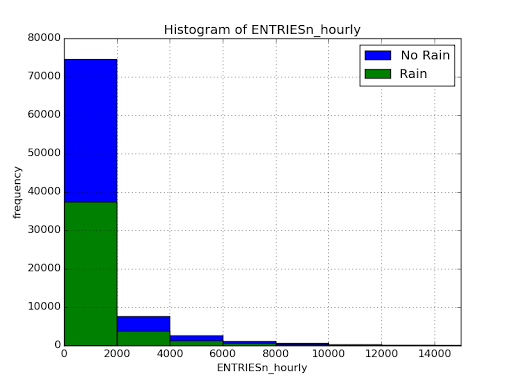
\includegraphics{ENTRIESn_hourly_distribution_3_1.png} This is of course
only one way to test for the normality of the data. We can also run a
Shapiro Wilks test on the data. This gives us a $ W = 0.475 $ and $ p
= 0.0 \textless{} 0.05 = p\_\{critical\} $ meaning we can reject the
null hypothesis of this data being normally distributed. However, as is
explained and shown very well in the link to the Shapiro Wilks Test,
this normality test can fail quite often and therefore looking at the
histograms might be a better way to ensure that the data is normally or
non-normally distributed.

Because the assumption of normallity is rejected we will be using the
\textbf{one-tailed Mann-Whitney U Test} with a $ p\_\{critical\} = 0.05
$.

\subsubsection{Statistical Test Results}\label{statistical-test-results}

Running the Mann-Whitney U Test on the data is done in problem set 3.3
in the Introduction to Data Science course. The two inputs to the
Mann-Whitney U Test are the ENTRIESn\_hourly for when it rains and when
it doesn't. The results of this test are:

\begin{longtable}[c]{@{}lll@{}}
\toprule
Statistic & Rain & No Rain\tabularnewline
\midrule
\endhead
\(\bar{x}_{ENTRIESn\_hourly}\) & 1105.4463767458733 &
1090.278780151855\tabularnewline
\bottomrule
\end{longtable}

and the U and p values returned from the scipy.stats.mannwhitneyu test
were:

\[ (U, p) \simeq (1924409167.0,\, 0.025) \]

    The scipy.stats.mannwhitneyu test returns the result of a
\textbf{one-tailed} test, but converting this to a two tailed is a
matter of multiplying by two. So our $ p = 0.024999912793489721
\simeq 0.025 $ for a one-tailed test is the same as a $ p =
0.04999982558697944 \simeq 0.05 $ for a two-tailed test. With a $
p\_\{critical\} = 0.05 $ we see that $ p \simeq 0.05 \textless{} 0.05
= p\_\{critical\} $ meaning we can reject the null hypothesis. The
significance of this test is that it shows that there are not the same
amount of people using the subway when it is and when it isn't raining.
From the reported means we can also see that the the distribution for
which it was raining is statistically greater than when it isn't. We
must however notice that the U value returned from the
scipy.stats.mannwhitneyu test is very large. Since smaller U values
indicate greater deviations from the null hypothesis, this large U value
indicates a very small deviation from the null hypothesis.

To try and predict the number of ENTRIESn\_houly I chose to use the
Statsmodels ordinary least squares linear regressor. OLS was chosen
because I found it to give better and more consistent results. The input
variables for the OLS model were \textbf{rain, precipi, meantempi,
maxpressurei, minpressurei, maxdewpti, fog, meanwindspdi, weekday, Hour,
rush\_hour, UNIT} The reason behind the inputs are different as some
were chosen because random testing showed them to have an effect on the
predictability of the model, whilst others were chosen because I
believed that these features had an effect on how well a model could
predict. * \textbf{Test chosen features:} rain, meanwindspdi, precipi,
meantempi, maxpressurei, minpressurei, maxdwpti, fog * \textbf{Reason
chosen features:} weekday, hour, rush\_hour, UNIT, warm, cold, dry,
moist, humid, windy

The test chosen features were found when testing the predictability and
adding features to try and find some improvement. Some features, like
maxpressurei, minpressurei, maxdwpti were added at random and were kept
because they turned out to increase predictability. Other features like
rain, meanwindspdi, precipi, and meantempi were added because I had the
idea that rain, wind and temperature would have an effect on how many
people would use the subway. Adding features based on ``raw'' data works
well to some degree. However, this is not always the best way to
increase predictability of a model. Oftentimes one can increase the
predictability vastly by either creating dummy variables, as was done
with the \textbf{UNIT} feature, or creating boolean features as was done
for the \textbf{weekday}, \textbf{rush\_hour}, \textbf{warm},
\textbf{cold}, \textbf{dry}, \textbf{moist}, \textbf{humid},
\textbf{windy} features. The dummy feature is a simple way to create
numeric features from non-numeric data, i.e.~going from categorical data
like the UNIT column which consists of names of the units which record
the ENTRIESn\_hourly, to \(N\) columns, where \(N\) is the number of
unique units. The boolean features were created because I believed that
there was a greater amount of people using the subway during the
weekdays than during the weekends, and also a greater amount of people
using the subway in what I call \emph{rush\_hour}, which is a time
interval from 10.00 (10am) to 22.00 (10pm). Furthermore all the weather
related boolean features were created because I assumed that more people
would use the subway during extreme(r) weather conditions (this actually
increased my \(R^2\) from 0.47 to about 0.5).

By using these features in the OLS the weights for the non-dummy
features were:

\begin{longtable}[c]{@{}lr@{}}
\toprule
Feature & Weight\tabularnewline
\midrule
\endhead
const & 14397.602439\tabularnewline
rain & -263.684249\tabularnewline
warm & -55.935904\tabularnewline
moist & 388.166843\tabularnewline
dry & 132.037170\tabularnewline
humid & -492.742290\tabularnewline
windy & -238.417431\tabularnewline
cold & -151.507613\tabularnewline
precipi & 209.676586\tabularnewline
maxpressurei & -653.533281\tabularnewline
minpressurei & 265.309983\tabularnewline
fog & 65.282306\tabularnewline
meanwindspdi & 26.384006\tabularnewline
weekday & 522.478287\tabularnewline
Hour & 24.224710\tabularnewline
meantempi & -31.054565\tabularnewline
maxdewpti & -5.279691\tabularnewline
rush\_hour & 696.724312\tabularnewline
\bottomrule
\end{longtable}

and the coefficient of determination returned was
\(R^2 = 0.499235384485 \simeq 0.5\). The point of the \(R^2\) is to give
an idea of how well the model fits the data. Because we have a
coefficient of determination of about \(0.5\) we can say that the model,
using the current features explains \(50\%\) of the variability of the
number of subway users. From my tests on the data set it seemed very
hard to increase the coefficient of determination above \(0.5\) and
therefore I believe that this model fits the data to the best of its
ability. Meaning that the model is somewhat succesful at predicting the
number of subway users, but that it might be a too simple model. Below
we also see a plot of the data and predictions done on the downloaded
dataset.

\begin{figure}[htbp]
\centering
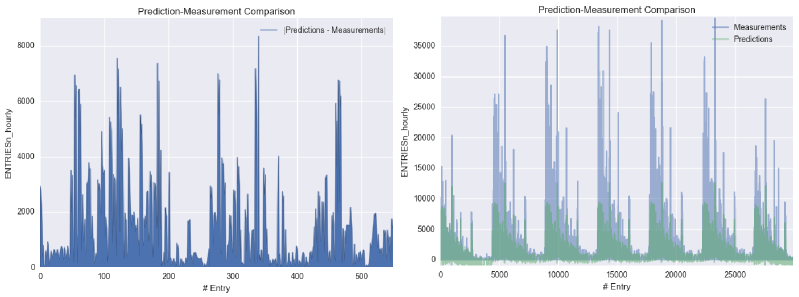
\includegraphics{prediction_measurement.png}
\caption{ENTRIESn\_hourly on prediction and measurement and difference}
\end{figure}

We have throughout the analysis of the NYC subway dataset tried to find
out if there are more people riding the NYC subway when it is raining
then when it isn't, and also tried to build a statistical machine
learning model to predict the number of subway users based on some
features of our own chosing/making. I believe that the best illustration
of whether or not more people ride the NYC subway when it is raining is
actually the first figure I show, which was the first analysis I did on
the data. On this figure we see the normalized NYC subway riders per
station/unit grouped into raining and not raining plotted on a map of
NY. I think it quite clearly shows that more people use the NYC subway
when it is raining than when it isn't. From this analysis there is also
another result, which might convey a more statistical way of indicating
a greater ridership when it is raing than when it isn't. This is the
result from the statistical test which showed that the null hypothesis,
of the number of subway users being the same when it was raining and
when it wasn't, could be rejected. However, we also see from the OLS
that the weight for the \textbf{rain} feature is negative! This could
mean that the \textbf{rain} feature has a negative effect on the number
of subway users, \textbf{or} it could be an effect of multicollinearity,
i.e.~that some of my features are highly linearly related. This is very
likely since e.g.~temperature, humidity, pressure and wind are all
highly correlated.

As a whole, I'm amazed at how much data is available if you just look
for it. This dataset inspired me to look at other datasets, and I found
many interesting public dataset, like the NYC taxi data. However there
are some things about this particular dataset which bothered me, and if
different might have resulted in a better model. Some shortcomings of
the dataset are the lack of consistent measurements. We have
measurements of ENTREISn\_hourly at various hours of the day, but there
is no continuous timeseries of measurements. I am well aware of the fact
that the data for ENTRIESn\_hourly is inherently discrete, but the lack
of consistent measurements bothered me. Some things I could've done
differently, was to visualize the data to try and find some patterns in
the data. This could've been done through clustering or grouping the
data. Furthermore, my analysis was done using a linear regression model,
but I strongly believe that the data is non-linear and that a non-linear
regressor could've performed better.


    % Add a bibliography block to the postdoc



    \end{document}
